\documentclass[11pt]{article}
\usepackage{amsmath, amssymb} %, graphicx}
\usepackage[pdftex]{graphicx}
\usepackage{subcaption}
\usepackage{units}
\usepackage{bm}
\usepackage[per-mode=symbol]{siunitx}

\usepackage[left=1in, right=1in, top=1in, bottom=1in]{geometry}
\usepackage{titling}


\title{Robot Learning DMP Assignment}
\author{Junhyeok Ahn}
\date{\today}
\begin{document}
\maketitle

%%%%%%%%%%%%%%%%%%%%%%%%%%%%%%%%%%%%%%%%%%%%%%%%%%%%%%%%%%%%%%%%%%%%%%%%%%%%%%
\section{Trajectory generation}
\label{sec:1}

I generated the trajectory using below equation:
\begin{equation}
    \label{eq:traj}
    \begin{split}
        x &= \frac{0.6}{\tau} t \\
        y &= A sin( \frac{2 \pi}{0.3} x),
    \end{split}
\end{equation}
where $A=0.15,~\tau=20$. I generated time stamps with
$0.1\si{\second}$ interval and got Cartesian $\mathbf{x}=(x,~y)$ trajectory
(Fig.~\ref{fig:time_even_traj}). Corresponding part in the code is 'gen\_demo'
function in the attached code. The demonstrated trajectory dataset is composed of
\begin{equation}
    \begin{split}
        \tau &= [(t_1,\mathbf{x}_{1}),~\cdots,~(t_n,\mathbf{x}_{2})],\\
        \mathbf{x}_{i} &= [x_i,~y_i]^\top.
    \end{split}
\end{equation}
\begin{figure}[htpb]
    \centering
    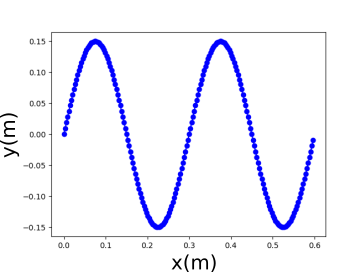
\includegraphics[width=0.5\linewidth]{figures/time_even_trajectory.png}
    \caption{ \textbf{Sine wave trajectory with identical time interval: }
    The trajectory starts from $[0,~0]^\top$ and ends at $[0.6,~0]^\top$ for
    $20$\si{\second}. Data are sampled with 0.1\si{\second} interval.}
    \label{fig:time_even_traj}
\end{figure}

%%%%%%%%%%%%%%%%%%%%%%%%%%%%%%%%%%%%%%%%%%%%%%%%%%%%%%%%%%%%%%%%%%%%%%%%%%%%%%
\section{DMP planning with linear interpolation}
\label{sec:dmp_learning_with_linear_interpolation}

I calculated
$\dot{\mathbf{x}},~\ddot{\mathbf{x}},~\mathbf{v},~\mathbf{\dot{v}}$ based on
the consecutive $ \mathbf{x} $'s in the trajectory $\tau$ and phase variable
$s$. Then I calculated $\mathbf{f}_{\rm target}(s)$ and appended it with corresponding
phase variable as below.
\begin{equation}
    \label{eq:dandf}
    \begin{split}
        \mathcal{D}&=[(s_1, \mathbf{f}_{\rm target,1}),~\cdots,~(s_n, \mathbf{f}_{\rm target,n})]\\
        \mathbf{f}_{\rm{target},i} &= [f_{\rm {target},i,x},~f_{\rm target,i,y}]^\top.
    \end{split}
\end{equation}
In this calculation, I used $\alpha=log(1-0.99)$ to make $s=0.01$ at the end.
Also, $K_p=1000,~K_d=600$ are used for both $x$ and $y$. In this problem, I
just copied all $\mathbf{f}_{target}(s)$ to $\mathbf{f}(s)=[f_x(s),~f_y(s)]$. Once
I got $\mathbf{f}(s)$, I planned the trajectory with the same start and goal
position with time interval $dt=0.001$. I queried the value $\mathbf{f}(s)$ at
every corresponding phase variables to forward integrate from starting
position. As the time stamps for new trajectory are not identical to the time
stamps in the demonstration trajectory $\tau$, I linearly interpolate to
compute $\mathbf{f}(s)$. The trajectory planned by DMP is shows in
Fig~\ref{fig:linear_interp}. In attached code, in DMP class, 'getPVA' function is
calculating velocity and acceleration and 'learn' function is learning DMP parameters,
such as $\mathbf{f}_{\rm target}$, weights for Gausian basis functions and so on.
In 'pred' function is used whenever I queried $\mathbf{f}$ at specific $s$.
Function 'plan' is the part actually planning using forward integration.
\begin{figure}[htpb]
    \centering
    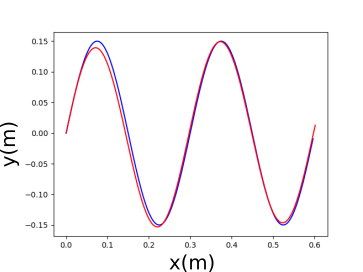
\includegraphics[width=0.5\linewidth]{figures/linear_interp.png}
    \caption{\textbf{DMP learning and planning with linear interpolation
    approximator: } Blue trajectory is demonstrated trajectory in
    Problem~\ref{sec:1} and red trajectory is planned from DMP using linear
    interpolation}
    \label{fig:linear_interp}
\end{figure}

%%%%%%%%%%%%%%%%%%%%%%%%%%%%%%%%%%%%%%%%%%%%%%%%%%%%%%%%%%%%%%%%%%%%%%%%%%%%%%
\section{Experiments with significantly differnt goals}
\label{sec:experiments_with_significantly_differnt_goals}

Based on the $\mathbf{f}(s)$ learned from $\mathbf{f}_{\rm target}(s)$ (in this
case I just copy this and linearly interpolated), I applied this motion
primitive to the different goals. In the attached code, different goals could
be easily specified by changing arguments.
\begin{figure}[htpb]
    \centering
    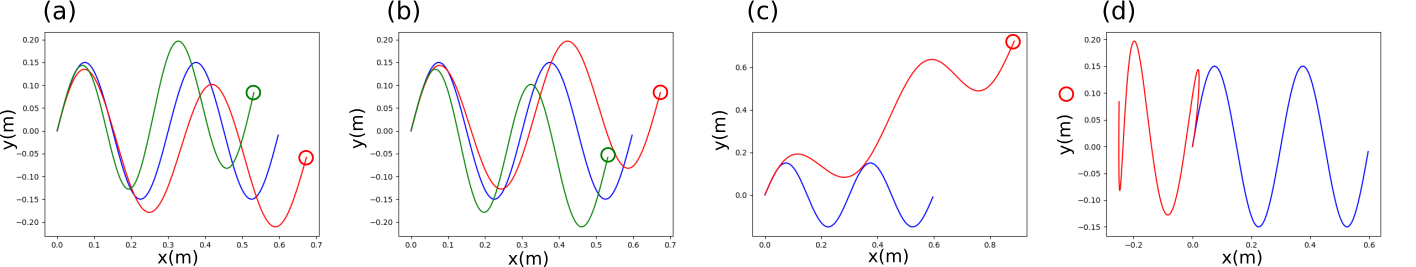
\includegraphics[width=\linewidth]{figures/another_goal.png}
    \caption{ \textbf{Experiments with different goals: }
    (a) red goal = $[0.7,~-0.1]^\top$, green goal = $[0.5,~0.1]^\top$
    (b) red goal = $[0.7,~0.1]^\top$, green goal = $[0.5,~-0.1]^\top$
(c) red goal = $[1.0,~0.9]^\top$ (d) red goal = $[-0.3,~0.1]^\top$  }
    \label{fig:different_goal}
\end{figure}
Figure~\ref{fig:different_goal} shows the planned trajectory from DMP with
different goals. (a), (b) and (c) show quite convergence compared to (d)
because nonlinear function behaves in the reverse direction in the case of the
goal located opposite direction.

\section{Experiments with various speed}
\label{sec:experiments_with_various_speed}
In this problem, I experimented with differnt temporal durations. In
Problem~\ref{sec:1}, I used $\tau=20$ for both demonstration and DMP planner.
To plan for half as fast and twice as fast trajectory from the same demonstration,
I maintained $\tau=20$ when I computed and approximated $\mathbf{f}_{\rm
target}$ and $\mathbf{f}_s$ but use $\tau=10$ and $20$ for the different time
durations in planning with DMP. Figure~\ref{fig:diff_speed} shows time versus
$x$ and $y$ and red trajectory represents planned with different time duration.
\begin{figure}[htpb]
    \centering
    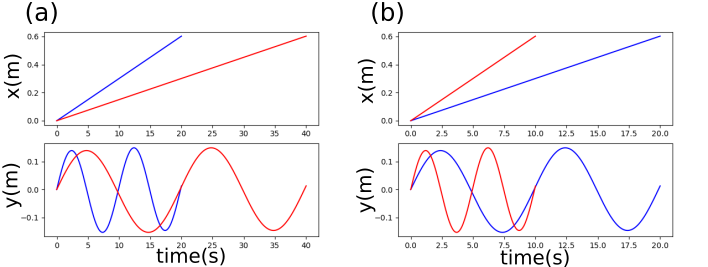
\includegraphics[width=0.7\linewidth]{figures/diff_speed.png}
    \caption{ \textbf{Trajectory planned by DMP with different time duration: }
    (a) shows the red trajectory planned for $\tau=40$, which is twice slower
    than blue. (b) shows the red trajectory planned for $\tau=20$, which is
    twice faster than blue.}
    \label{fig:diff_speed}
\end{figure}

\section{Generate trajectory with Gaussian noise}
\label{sec:generate_trajectory_with_gaussina_noise}
Similar to Problem~\ref{sec:1}, I generated one trajectory $\tau_1$, and add
Gaussian noise $\mathcal{N}(0,~1) / c$ to $x$ and $y$, where c is a scaling
factor. Figure~\ref{noise} shows the original trajectory and differentiated
trajectory with gaussian noise. I used $c=250$ as the scaling factor.
\begin{figure}[htpb]
    \centering
    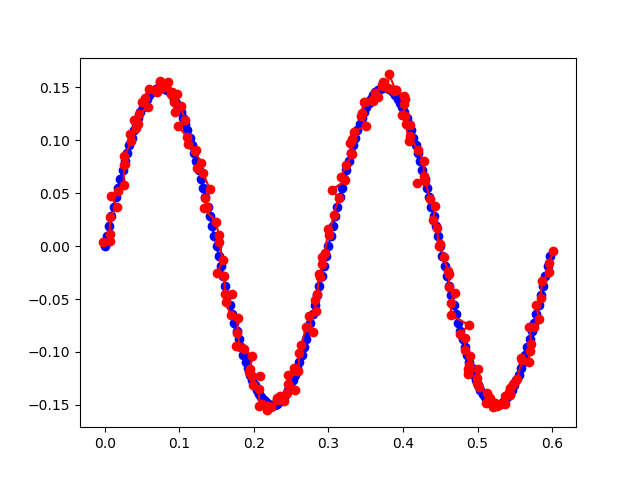
\includegraphics[width=0.5\linewidth]{figures/noise.png}
    \caption{ \textbf{Trajectory with Gaussian noise: } Blue and red trajectories
    are both demonstrated trajectory. However, red trajectory includes Gaussian
    noises}
    \label{noise}
\end{figure}

\section{DMP planning with Radial Basis Function}
\label{sec:dmp_planning_with_radial_basis_function}

Based on the trajectories in Figure~\ref{noise}, I calculated $\mathbf{f}_{\rm target}$
in similar way to Problem~\ref{sec:dmp_learning_with_linear_interpolation} for both trajectory and
generated dataset $\mathcal{D} = \{(s_1,~\mathbf{f}_{\rm target,1}),~\cdots,~(s_n,~\mathbf{f}_{\rm
target,n})\}$. I multiplied $\Sigma_{i} \frac{\psi_{i}(s)}{s}$ to transform
problem into the standard regression problem as
\begin{equation}
    \label{eq:lp}
    \begin{bmatrix}
        \mathbf{f}_{\rm target,1}(s)\Sigma_{i} \frac{\psi_{i}(s_1)}{s_1} \\ \vdots \\ \mathbf{f}_{\rm target,n}(s)\Sigma_{i} \frac{\psi_{i}(s_n)}{s_n}
    \end{bmatrix}
    =
    \begin{bmatrix}
        \psi_{1,1}(s_1) & \cdots & \psi_{1, m}(s_1) \\
        \vdots     & \ddots & \vdots      \\
        \psi_{n,1}(s_n) & \cdots & \psi_{n, m}(s_n)
    \end{bmatrix}
    \begin{bmatrix}
        w_1 \\ \vdots \\ w_n
    \end{bmatrix},
\end{equation}
where n and m is the number of datapoint and basis functions respectively. Note
that $\mathbf{f}_{\rm target} \in \mathbb{R}^2$ as defined in
Eq.~\eqref{eq:dandf}, so I solved Eq.~\eqref{eq:lp} twice for $x$ and $y$.
Then, using left pseudo inverse, weights could be computed as,
\begin{equation}
    \begin{bmatrix}
        w_1 \\ \vdots \\ w_n
    \end{bmatrix} =
    \left( \Psi^\top \Psi \right)^{-1} \Psi^\top
    \begin{bmatrix}
        \mathbf{f}_{\rm target,1}(s)\Sigma_{i} \frac{\psi_{i}(s_1)}{s_1} \\ \vdots \\ \mathbf{f}_{\rm target,n}(s)\Sigma_{i} \frac{\psi_{i}(s_n)}{s_n}
    \end{bmatrix}.
\end{equation}
In here I used 40 Gaussian functions for each $x$ and $y$ to approximate $\mathbf{f}(s)$.
Once the weights are calculated, I could forward integrate to the trajectory.
The trajectory from the DMP is illustrated in Figure~\ref{fig:figures/rbf}.
\begin{figure}[htpb]
    \centering
    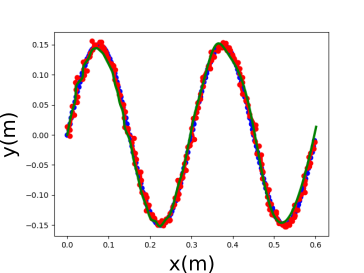
\includegraphics[width=0.5\linewidth]{figures/rbf}
    \caption{ \textbf{DMP learning and planning with radial basis function
    approximator: } Green trajectory is planned from DMP using radial basis
    functions. 40 basis functions are used to approximate $\mathbf{f}(s)$ for
    each $x$ and $y$.}
    \label{fig:figures/rbf}
\end{figure}

Now, I will show several trials I played with number of basis functions and
placing the center of radial basis functions.
Figure~\ref{fig:figures/different_s} shows unevenly distributed center case and
evenly distributed center case respectively.  It is able to see putting phase
variable $s$ more around $0 \sim 0.5$ shows better result. This is because the
demonstrated data is more densly distributed where s is close to 0.  Therefore, the
final parameters I've use is 40 basis functions (put 20 between $0\sim0.5$ and
put the others 20 between $0\sim1$) with $1500$ width.
\begin{figure}[htpb]
    \centering
    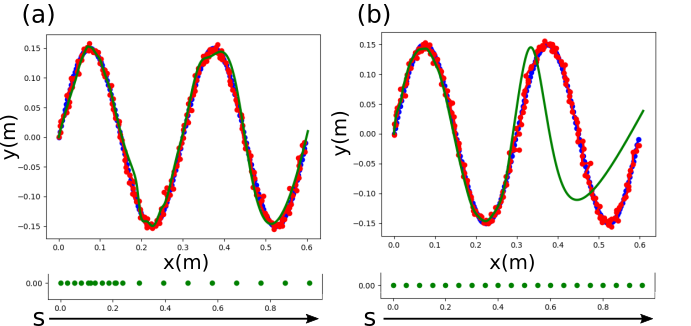
\includegraphics[width=0.7\linewidth]{figures/different_s.png}
    \caption{ \textbf{Comparing two different planned trajectory with
    different radial basis function center: } (a) shows 20 unevenly distributed
    centers. (b) shows 20 evenly distributed centers. green dots represents the center
    of radial basis functions. Note that to show the different clearly I only
    used 20 basis functions even though I used 40 basis functions for the others.}
    \label{fig:figures/different_s}
\end{figure}

I also described how DMP with radial basis functions generalize the different
goals. It generalized trajectories with different goals in Fig.~\ref{different_goals_2}.
\begin{figure}[htpb]
    \centering
    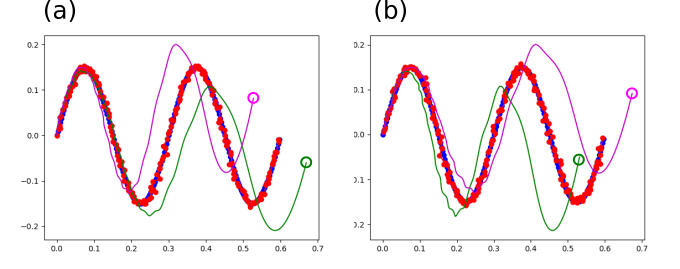
\includegraphics[width=0.7\linewidth]{figures/different_goals_2.png}
    \caption{ \textbf{Experiments with different goals: } (a) pink goal =
    $[0.5,~0.1]^\top$, green goal = $[0.7,~-0.1]^\top$(b) pink goal =
    $[0.7,~0.1]^\top$, green goal = $[0.5,~-0.1]^\top$}
    \label{different_goals_2}
\end{figure}
\section{Obstacle Avoidance}
\label{sec:obstacle_avoidance}
I placed an obstacle at $\mathbf{p}_{obs}=[0.21,~0.0]^\top$ which is
exerting an acceleration, which is weakened with distance
as a Gaussian that is strongest at the obstacle center
\begin{align}
    %r &= \lvert \lvert\mathbf{x} - \mathbf{p_{obs}} \rvert \rvert_{2}, \\
    r &= \sqrt{(x - p_{obs, x})^2 + (y - p_{obs, y})^2}, \\
    \theta &= arctan2(y - p_{obs, y},~x - p_{obs, x}), \\
    \rm acc_{\rm obs} &= 50e^{-100(r-0)^2}[cos\theta,~ sin\theta]^\top,
\end{align}
where $\mathbf{x}$ and $\mathbf{p}_{\rm obs}$ are position of robot (end
effector in Cartesian) and obstacle respectively and $\rm acc_{\rm obs}$ is
added on the trajectory. I also used scaler factor 50. Figure~\ref{fig:obs}
shows the red trajectory trying to avoid the obstacle.
\begin{figure}[htpb]
    \centering
    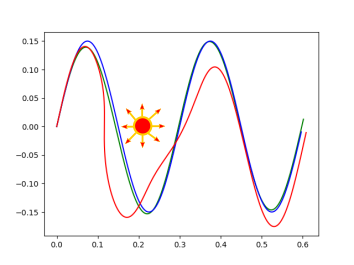
\includegraphics[width=0.5\linewidth]{figures/obs.png}
    \caption{ \textbf{Obstacle avoidance: } blue trajectory is demonstrated and
    green trajectory is planned trajectory without obstacle. Obstacle is placed
    at $[0.21,~-0.13]^\top$ and the resulting trajectory is illustrated as red.}
    \label{fig:obs}
\end{figure}

\section{Additional Questions}

\subsection{Under what condition DMP works well or not}
As demonstrated in Figure~\ref{fig:different_goal}, DMP could generalize
trajectory quite well in the case that the new goal is located in the same side
of the goal demonstrated. For example, if I look at the (a) and (b), the
trajectory almost converges to the goal with maintaining the primitive of the
demonstrated trajectory. Even though there is some slight error at the goal,
(c) shows the similar trends in the trajectory. However, if I look at (d),
x axis goal lays in the opposite side but, y axis goal is not located so far.
The trajectory planned from DMP shows a big error in $x$ compared to $y$.
Therefore, I could conclude the goal location affects the performance of
convergence as well as the similarity on the shape (or primitive).

Also, DMP is not converged if the obstacle is located near the goal. It is quite
obvious because it is generating an acceleration. Figure~\ref{fig:obs_near_goal}
shows the case I put obstacle at the goal position $[0.6,~0]^\top$.
\begin{figure}[htpb]
    \centering
    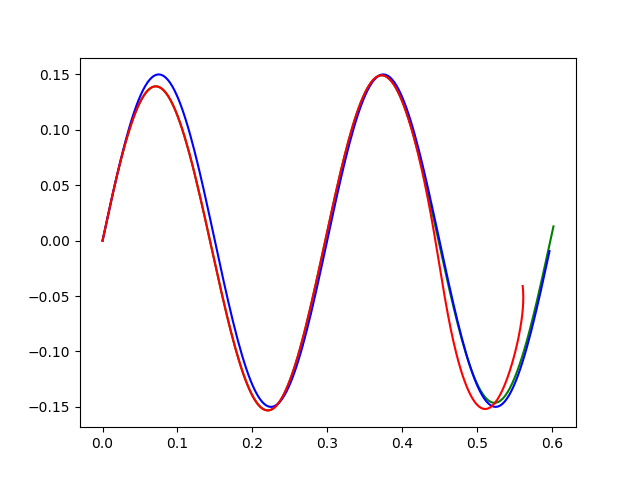
\includegraphics[width=0.5\linewidth]{figures/obs_at_goal.png}
    \caption{ \textbf{Obstacle at goal position: } The obstacle is located at
    goal position where $[0.6,~0]^\top$. The green trajectory shows the planned one
    without obstacle and the red shows the trajectory considering obstacle}
    \label{fig:obs_near_goal}
\end{figure}

\subsection{How to respond to perturbation}
The easiest way to implement DMP robust to the perturbation is to use large
$K_p$ and $K_d$ gain and makes phase variable $s$ converge to zero quickly.
This will reduce a tendency to follow up the trajectory demonstrated and improve
convergence to the goal. Also, I could also update $f(s)$ whenever the trajectory
is executed.

\subsection{Which parameters could be perturbed to improve performance}
If I assume the cost/reward function is well described, now the problem is more
than minimizing the error between $f(s)$ and $f_{target}$. Because demonstration
should not be illustrating the trajectory in terms of well described cost. So
the weights as well as the center and width of radial basis function are all
subject to be perturbed.



\end{document}

